\documentclass{standalone}
\usepackage{amsmath,amssymb}
\usepackage{tikz-cd}
\begin{document}
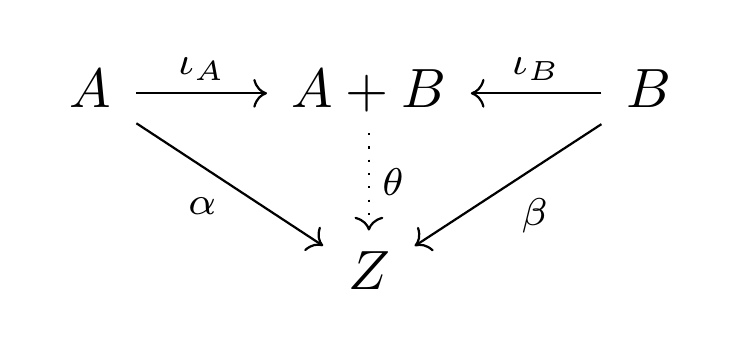
\begin{tikzpicture}[baseline= (TIKZCD).base]
\node[scale=2] (TIKZCD) at (0,0){
\begin{tikzcd}
A \arrow[r, "\iota_A"] \arrow[dr, "\alpha"'] & A + B \arrow[d, dotted, "\theta"] & B \arrow[l, "\iota_B"'] \arrow[dl, "\beta"] \\
& Z &
\end{tikzcd}
};
\end{tikzpicture}
\end{document}
